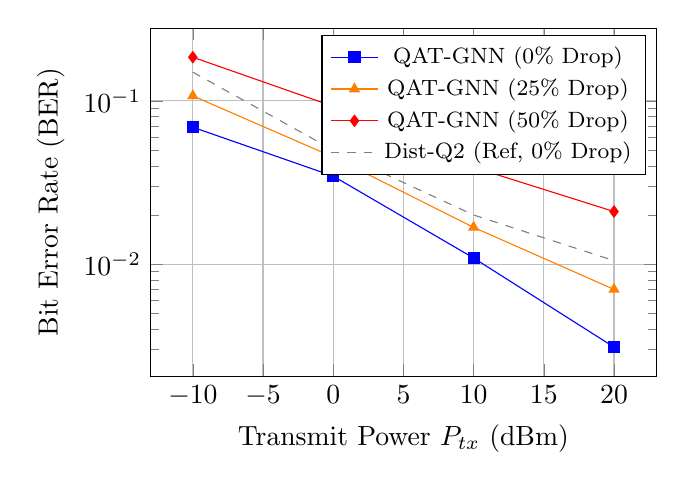
\begin{tikzpicture}
\begin{semilogyaxis}[
    xlabel={Transmit Power $P_{tx}$ (dBm)},
    ylabel={Bit Error Rate (BER)},
    grid=major,
    legend style={at={(0.98,0.98)}, anchor=north east, font=\footnotesize},
    width=8cm,
    height=6cm
]

% QAT-GNN 0% Drop
\addplot[color=blue, mark=square*] coordinates {
    (-10, 0.0690) (0, 0.0346) (10, 0.0109) (20, 0.0031)
};
\addlegendentry{QAT-GNN (0\% Drop)}

% QAT-GNN 25% Drop
\addplot[color=orange, mark=triangle*] coordinates {
    (-10, 0.1074) (0, 0.0453) (10, 0.0168) (20, 0.0070)
};
\addlegendentry{QAT-GNN (25\% Drop)}

% QAT-GNN 50% Drop
\addplot[color=red, mark=diamond*] coordinates {
    (-10, 0.1853) (0, 0.0926) (10, 0.0392) (20, 0.0210)
};
\addlegendentry{QAT-GNN (50\% Drop)}

% Reference Dist-Q2 (0% Drop) for context
\addplot[color=gray, mark=none, dashed] coordinates {
    (-10, 0.15) (0, 0.05) (10, 0.02) (20, 0.0105)
};
\addlegendentry{Dist-Q2 (Ref, 0\% Drop)}

\end{semilogyaxis}
\end{tikzpicture}